\documentclass[12pt,a4paper]{article}
\usepackage{ctex}
\usepackage{amsmath,amscd,amsbsy,amssymb,latexsym,url,bm,amsthm}
\usepackage{epsfig,graphicx,subfigure}
\usepackage{enumitem,balance}
\usepackage{wrapfig}
\usepackage{mathrsfs,euscript}
\usepackage[usenames]{xcolor}
\usepackage{hyperref}
\usepackage[vlined,ruled,linesnumbered]{algorithm2e}
\usepackage{array}
\hypersetup{colorlinks=true,linkcolor=black}

\newtheorem{theorem}{Theorem}
\newtheorem{lemma}[theorem]{Lemma}
\newtheorem{proposition}[theorem]{Proposition}
\newtheorem{corollary}[theorem]{Corollary}
\newtheorem{exercise}{Exercise}
\newtheorem*{solution}{Solution}
\newtheorem{definition}{Definition}
\theoremstyle{definition}

\renewcommand{\thefootnote}{\fnsymbol{footnote}}

\newcommand{\postscript}[2]
 {\setlength{\epsfxsize}{#2\hsize}
  \centerline{\epsfbox{#1}}}

\renewcommand{\baselinestretch}{1.0}

\setlength{\oddsidemargin}{-0.365in}
\setlength{\evensidemargin}{-0.365in}
\setlength{\topmargin}{-0.3in}
\setlength{\headheight}{0in}
\setlength{\headsep}{0in}
\setlength{\textheight}{10.1in}
\setlength{\textwidth}{7in}
\makeatletter \renewenvironment{proof}[1][Proof] {\par\pushQED{\qed}\normalfont\topsep6\p@\@plus6\p@\relax\trivlist\item[\hskip\labelsep\bfseries#1\@addpunct{.}]\ignorespaces}{\popQED\endtrivlist\@endpefalse} \makeatother
\makeatletter
\renewenvironment{solution}[1][Solution] {\par\pushQED{\qed}\normalfont\topsep6\p@\@plus6\p@\relax\trivlist\item[\hskip\labelsep\bfseries#1\@addpunct{.}]\ignorespaces}{\popQED\endtrivlist\@endpefalse} \makeatother

\begin{document}
\noindent

%========================================================================
\noindent\framebox[\linewidth]{\shortstack[c]{
\Large{\textbf{Lab09-Network Flow}}\vspace{1mm}\\
CS214-Algorithm and Complexity, Xiaofeng Gao \& Lei Wang, Spring 2021.}}
\begin{center}
\footnotesize{\color{red}$*$ If there is any problem, please contact TA Yihao Xie. }

\footnotesize{\color{blue}$*$ Name:RenyangGuan  \quad Student ID:519021911058 \quad Email: guanrenyang@sjtu.edu.cn}
\end{center}

\begin{enumerate}
    \item  Consider there is a network consists $n$ computers. For some pairs of computers, a wire $i$ exists in the pair, which means these two computers can communicate with each other. When a signal passes through the wires, the noise in the signal will be amplified.If you know the magnification rate of noise $m_{i,j}$ of each wire (which must be greater than 1). Design an algorithm to find the route  for each other computer to send signals to the computer $v$ with the minimum total magnification rate of noise and analyze the time complexity.
	\begin{solution}
	In graph $G=(V,E)$, let $v\in V$ denote each computer and $e\in E$ denote the wire between computers. 
	\\
	\textbf{\textit{Intuition:}}
	The intuition comes from $Dijkstra$ algorithm and is based on $Greedy$ algorithm. 
	\\
	Firstly, we should re-define the shortest path as the path in which the product of the weight of each path is the minimum.
	\\
	Then we maintain a set $S$ of vertices whose shortest path distance from $S$ are known. At each step add to $S$ the vertex $v\in V-S$ whose distance estimate for $S$ is minimal, Finally, update the distance estimates of vertices adjacent to $v$.
	\\
	Since each wire is able to sent or receive signals, so $G$ is an undirected graph. The shortest path of $(u,v)$ is the same as that of $(v,u)$. As a result of this, setting the sink vertex $v$ as the source vertex in the $Modified Dijkstra$ algorithm could get the result.
	\\
	\begin{algorithm}[H]
	        \caption{Modified Dijkstra Algorithm}\label{Alg-SHORSTPATH}
	        \KwIn{object vertex $v$ receiving signals}
	        \KwOut{An array $d$ maintaining result }
	
	        \BlankLine
	        create array $d$\;
            create min-heap $Q$\;
            \BlankLine
            \ForEach{$k\in V$}{
                \If{$k=v$}{
                    $d[k]\leftarrow 0$\;
                }
                \Else{
                $d[k]\leftarrow \infty$\;}
            }
            \BlankLine
	        \ForEach{$u\in V$}{
	            $INSERT(Q,d[u])$\;
	        }
	        \While{$Q\neq \emptyset$}{
	            $u\leftarrow$ EXTRACT-MIN($Q$)\;
	            $S\leftarrow S\cup \{u\}$\;
	            \ForEach{$v\in adjacent(u)$}{
	                \If{$d[v]>d[u]\times w(u,v)$}{
	                    $d[v]\leftarrow d[u]\times w(u,v)$\;
	                    DECREASE-KEY$(Q,d[v])$\;
	                }
	            }
	        }
    \end{algorithm}
    \textbf{Time complexity algorithm:}
    The $for$ loop in line 3, the $for$ loop in line 8, and the $while$ loop in line 10 will loop for $|V|$ times. The time complexity of $INSERT$ and that of $DECREASE-KEY$ are based on the data structure of $Q$, as well as the density of the graph. 
    By using the best data structure Fibonacci heap, the time complexity could be reduced to $O(|V|\log |V|+|E|)$.
    \\
    Considering the density, since $|E|\leq\frac{|V|(|V|-1)}{2}$, the total time complexity won't exceed $O(|V|^2)$
    \\
    
	\end{solution}
	\item Suppose that we wish to maintain the transitive closure of a directed graph $G=(V,E)$ as we insert edges into $E$. That is, after each edge has been inserted, we want to update the transitive closure of the edges inserted so far. Assume that the graph $G$ has no edges initially and that we represent the transitive closure as a boolean matrix.
	\begin{enumerate}
	    \item Show how to update the transitive closure of a graph $G=(V,E)$ in $O(V^2)$ time when a new edge is added to $G$.
	    \item Give an example of a graph $G$ and an edge $e$ such that $\Omega(V^2)$ time is required to update the transitive closure after the insertion of $e$ into $G$, no matter what algorithm is used.
	    \item Describe an efficient algorithm for updating the transitive closure as edges are inserted into the graph. For any sequence of $m$ insertions, your algorithm should run in total time $\sum_{i=1}^m t_i=O(V^3)$, where $t_i$ is the time to update the transitive closure upon inserting the $i$th edge. Prove that your algorithm attains this time bound.
	\end{enumerate}
	\begin{solution}
	~\\
	~\\
	    \textbf{\textit{Notation:}}
	    \\
	    In graph $G=(V,E)$, let boolean matrix $A=(a_{ij})_{|V|\times |V|}$ to maintain the transitive closure, in which $a_{ij}=1$ means there exists a directed path from vertex $v_i$ to $v_j$.
	    \\
	    \\
	    \textbf{\textit{Algorithm pseudocode:}}
	    \\
	    \begin{algorithm}[H]
	        \caption{$INSERT(v_i,v_j,A)$}\label{Alg-INSERT}
	        \KwIn{An edge from $v_i$ to $v_j$, matrix $A$}
	        \KwOut{Boolean martix $A$ maintaining the transtive closure}
	
	        \BlankLine
	        
	        Create array $Source=\{0\}$, $Sink=\{0\}$\;
	        
	        $a_{ij}=1$\;
	        \ForEach{$ v_k\in\ V$ }
	        {
	            \If{$a_{ki}=1$ and $a_{kj}\neq 1$}
	            {
	                $Source\leftarrow k$\;
	            }
	            \Else
	            {
	                $Sink\leftarrow k$\;
	            }
	        }
	        \ForEach{$i\in\ Source$}
	        {
	            \ForEach{$j\in Sink$}
	            {
	                $a_{ij}\leftarrow 1$\;
	            }
	        }
	    \end{algorithm}
	   
    \textbf{\textit{Example:}}
    \begin{figure}[!htbp]
        	\centering
        	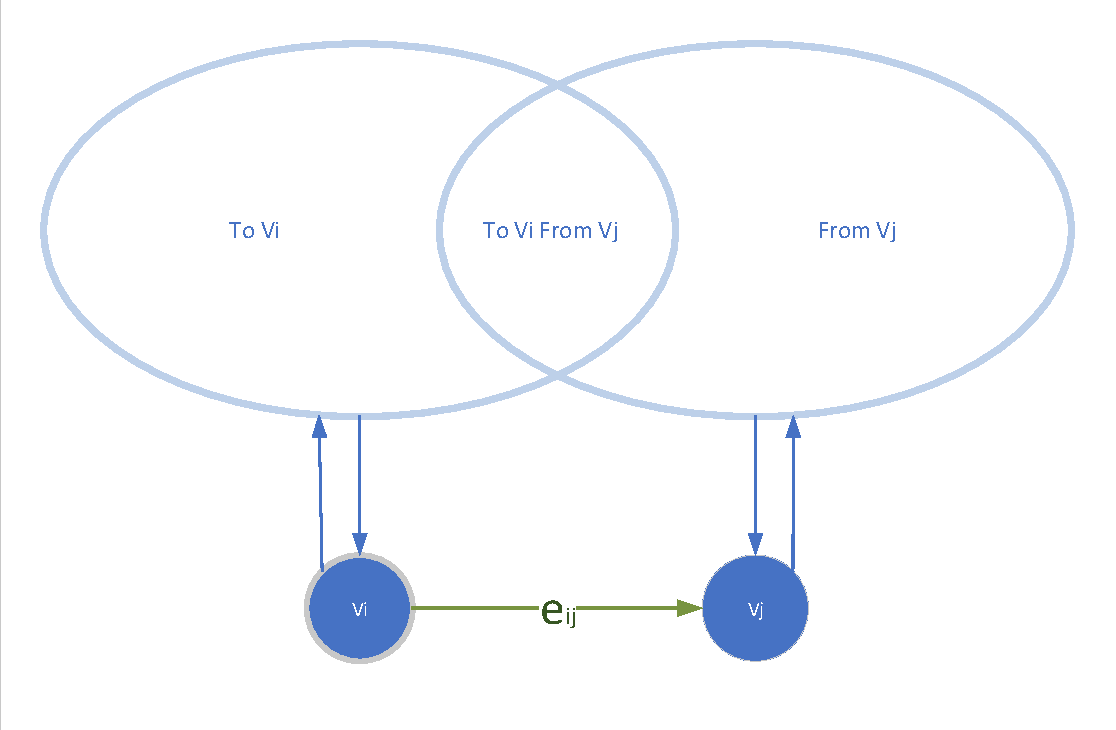
\includegraphics[width=0.6\textwidth]{Fig-EXAMPLE.pdf}
        	\caption{The example for time complexity of insertion}
        	\label{Fig-EXAMPLE}
    	\end{figure}
    As is shown in Fig.~\ref{Fig-EXAMPLE}, for each inserted edge $e$ from $v_i$ to $v_j$, we must check each node to determine whether it has a path toward $v_i$ or a path coming from $v_j$, which takes $O(|V|)$ time. 
    Let set $ToVi$ denote the set of vertices having a path to $v_i$ and $FromVj$ denote the set of vertices having a path from $v_j$. For any $p,q$, where $v_p\in ToVi$ and $v_q\in FromVj$, there exists a path from $v_p$ to $v_q$. As a result, we must update $a_{pq}$ which takes time $\Theta (|ToVi|\times|FromVj|)$. On average, $ToVi\sim V$ and $FromVj\sim V$, so the time complexity is at least $\Omega (|V|^2)$
    
    \textbf{\textit{Time complexity analysis:}}
	Since the graph $G$ is empty initially, the sequence of $m$ operation will all at most $m$ edges. Additionally, the number of edges is at most $\frac{|V|\times (|V|-1)}{2}$, which is the possible range of $m$.
	\\
	\textit{Case 1:} $m=O(|V|)$. Since the worst case time complexity of a single operation is $O(|V|^2)$, the total time complexity of the sequence of $m$ operations is $O(|V|^3)$.\\
	\textit{Case 2:} $m=O(|V|^2)$. Only when $a_{ki}=1$ and $a_{kj}\neq 1$, vertex $k$ will be added into $Source$. The same is $Sink$. In such case, the time complexity of the $for$ loop in the line 8 is $O(|V|)$ and total time complexity is $O(|V|)$ \\
	When the number of edges of $G$ is equivalent of $\Omega(|V|)$, the number of operations where $|Source|\sim O(|V|)$ and $|Sink|\sim O(|V|)$ is $\Theta(1)$. 
	As a result of this, the amortized total time complexity is
	$$O(|V|)\times \Theta(|V|^2)+O(|V|^2)\times \Theta(|V|)=O(|V|^3)$$
	\end{solution}
	\item An $n\times n$ grid is an undirected graph consisting of n rows and n columns of vertices, as shown in Figure 26.11. We denote the vertex in the $i$th row and the $j$th column by $(i,j)$. All vertices in a grid have exactly four neighbors, except for the boundary vertices, which are the points $(i,j)$ for which $i = 1, i = n, j = 1$, or $j = n$.
    Given $m\leqslant n^2$ starting points $(x_1,y_1), (x_2, y_2), ... , (x_m, y_m)$ in the grid, the escape problem is to determine whether or not there are $m$ vertex-disjoint paths from the starting points to any $m$ different points on the boundary such that every vertex in $V$ is included in at most one of the $m$ paths. For example, the grid in Figure \ref{Fig-EscapeProblem}(a) has an escape, but the grid in \ref{Fig-EscapeProblem}(b) does not.
    \begin{figure}[!htbp]
	\centering
	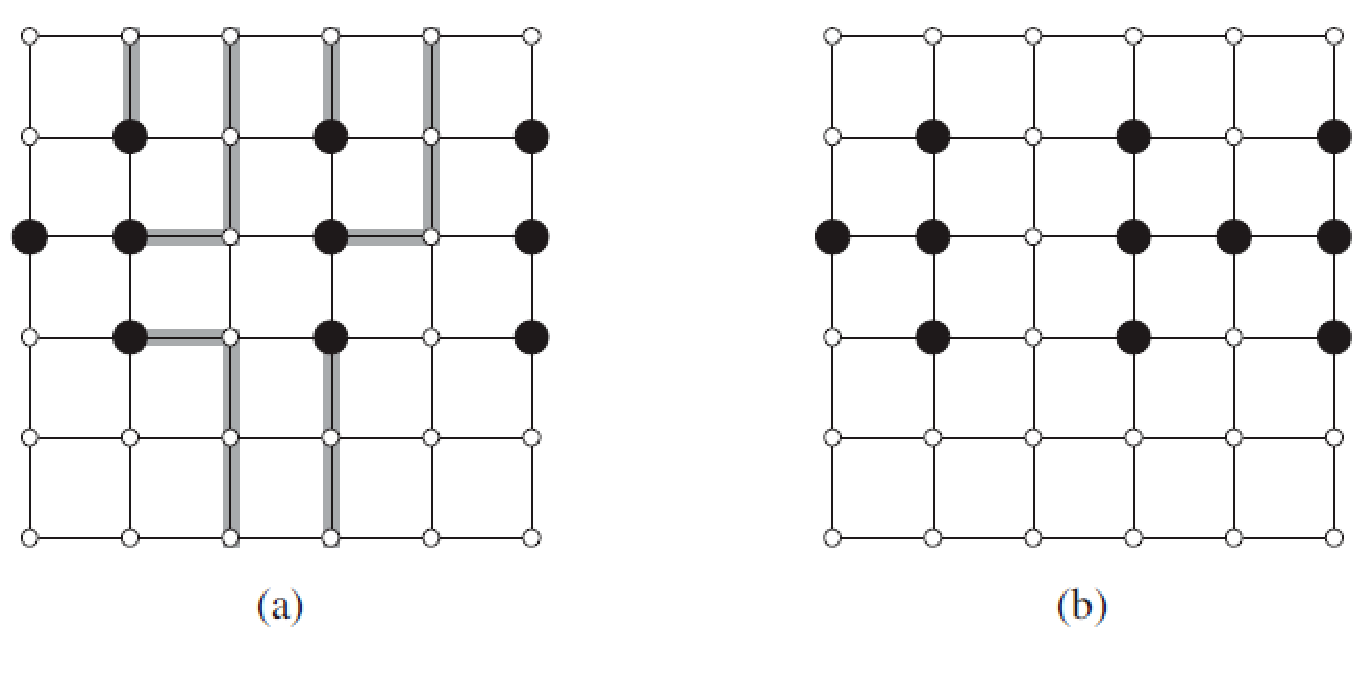
\includegraphics[width=0.5\textwidth]{Fig-EscapeProblem.pdf}
	\caption{Grids for the escape problem. Starting points are black, and other grid vertices are white. (a) A grid with an escape, shown by shaded paths. (b) A grid with no escape.}
	\label{Fig-EscapeProblem}
	\end{figure}
	
    \begin{enumerate}
        \item Consider a flow network in which vertices, as well as edges, have capacities. That is, the total positive flow entering any given vertex is subject to a capacity constraint. Show that determining the maximum flow in a network with edge and vertex capacities can be reduced to an ordinary maximum-flow problem on a flow network of comparable size. That is, the sizes of the two graph are in the same order of magnitude.
        \item Describe an efficient algorithm to solve the escape problem, and analyze its running time.
    \end{enumerate}
    \begin{solution}
    ~\\
    \begin{enumerate}
        \item [(a)]
        Transforming the network with vertices as well as edges having capacities into ordinary network could be done by \emph{splitting} vertices.
        \\
        Let $v$ be the vertex with capacity $w_v$.
        The \emph{split} operation is shown in Fig.~\ref{Fig-P3T1}. 
        \\
        \begin{enumerate}
            \item Delete the vertex $v$ and add two vertices $v_i$, $v_j$ with infinity capacity.
            \item Add edge $e_{ij}$ from $v_i$ to $v_j$ with capacity $W_v$ into $G$.
            \item For each edge $e_{u,v}$ from vertex $u$ to $v$, traverse it to $e_{u,v_i}$. Similarly, traverse each out-edge $e_{v,k}$ to $e_{v_j,k}$.
        \end{enumerate}
        \begin{figure}[!htbp]
        	\centering
        	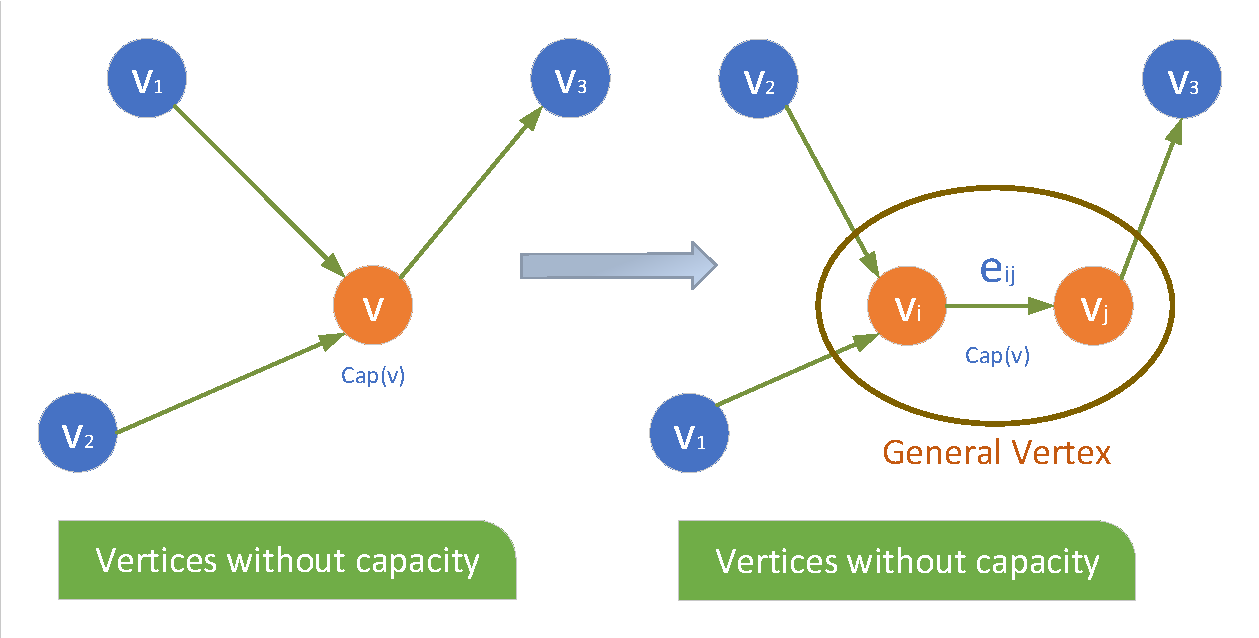
\includegraphics[width=0.6\textwidth]{Fig-P3T1.pdf}
        	\caption{Transform the question into ordinary network flow}
        	\label{Fig-P3T1}
    	\end{figure}
    	\textbf{\textit{Correctness:}}
    	\\
    	The transforming method maintains the twp properties of flow network.
        \begin{enumerate}
            \item The capacity of each remaining edge is maintained.
            \item Each edge is transformed into general vertex. The in-flow and out-flow of each general vertex is the same as before. The edge in the general edge constraint the capacity of it.
        \end{enumerate}
    \item[(b)] ~\\
    \textbf{\textit{Step 1:}} Delete starting points in the boundary, as is shown in Fig.~\ref{Fig-STEP1}. 
    \\
    Firstly we should delete the starting points in the boundary, because it could be neither the ending point nor the middle point of a path. Additionally, the edge connecting this kind of  vertex and the inner vertex can never be passed by. As a result of this, deleting it makes sense.
    \begin{figure}[!htbp]
	\centering
	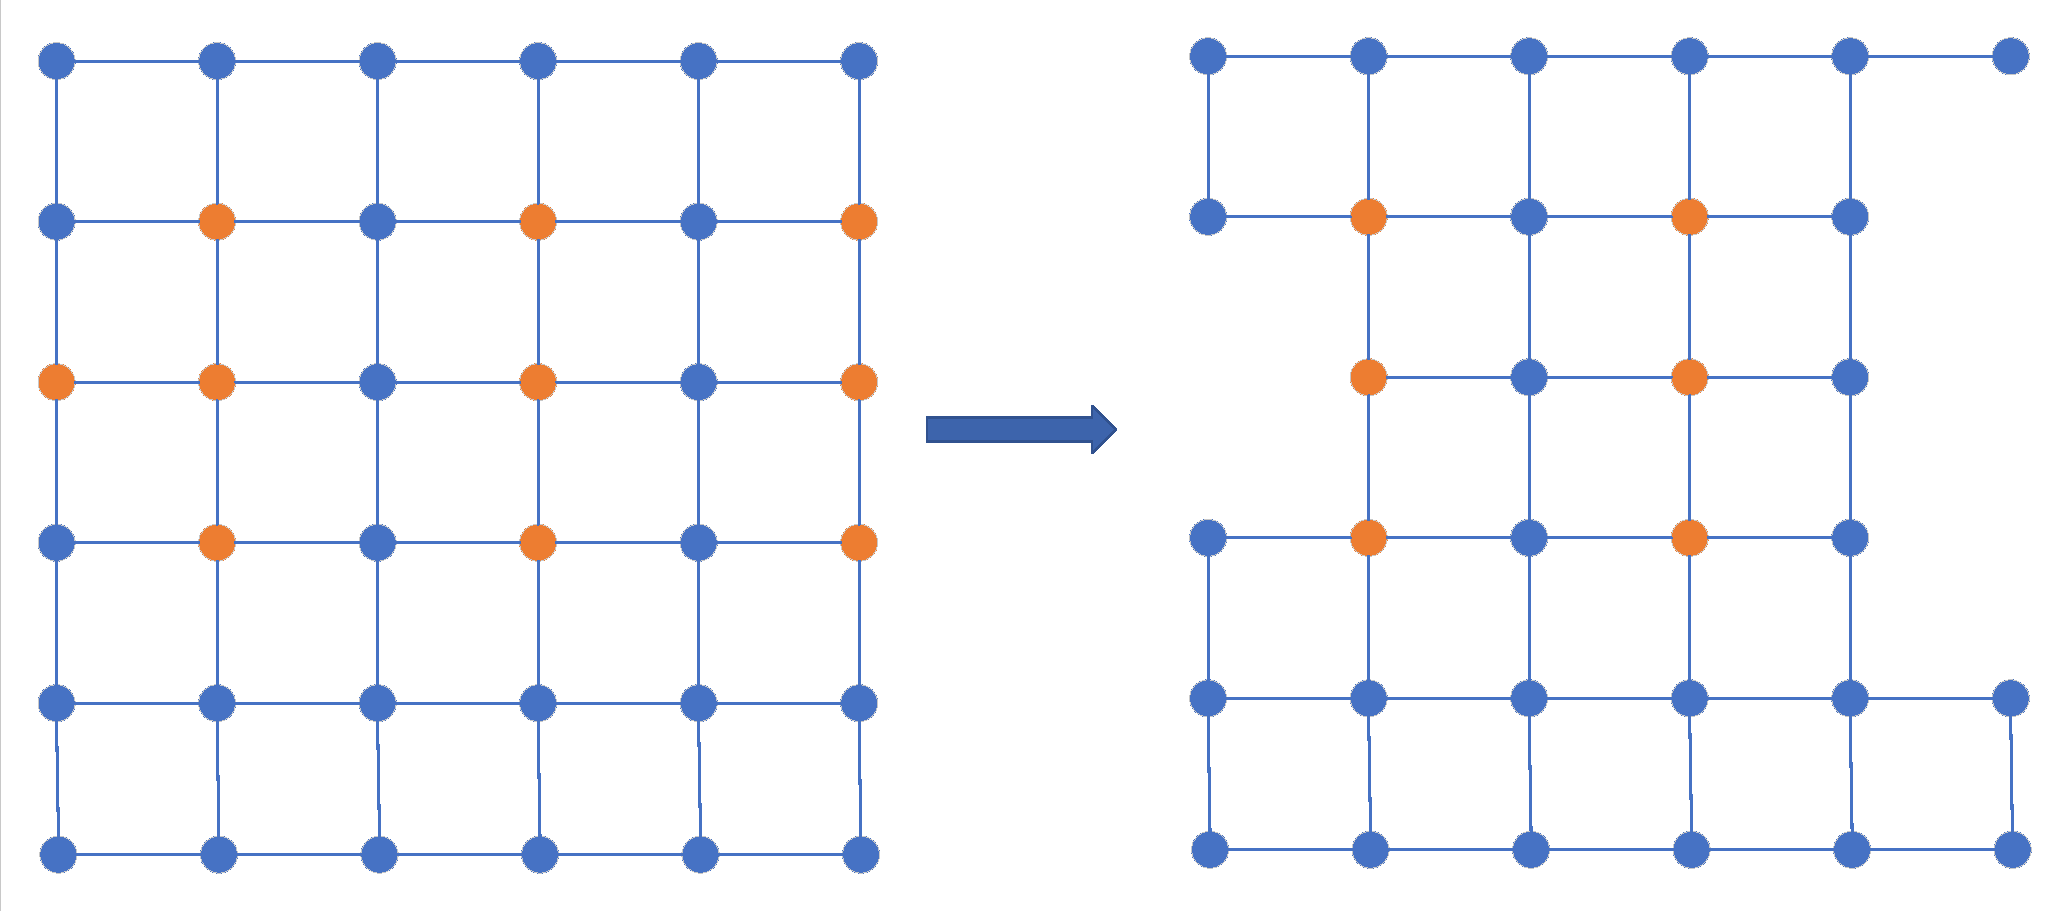
\includegraphics[width=0.5\textwidth]{Fig-P3T2SETP1.pdf}
	\caption{Step1: Delete starting points in the boundary.}
	\label{Fig-STEP1}
	\end{figure}
	\\
	\textbf{\textit{Step 2:}} Abstract the boundary into one node, as is shown in Fig.~\ref{Fig-STEP2}. 
    \\
    Abstract the remaining outer vertices into one vertex with each vertex in the sub outer layer having an edge into it.
    \begin{figure}[!htbp]
	\centering
	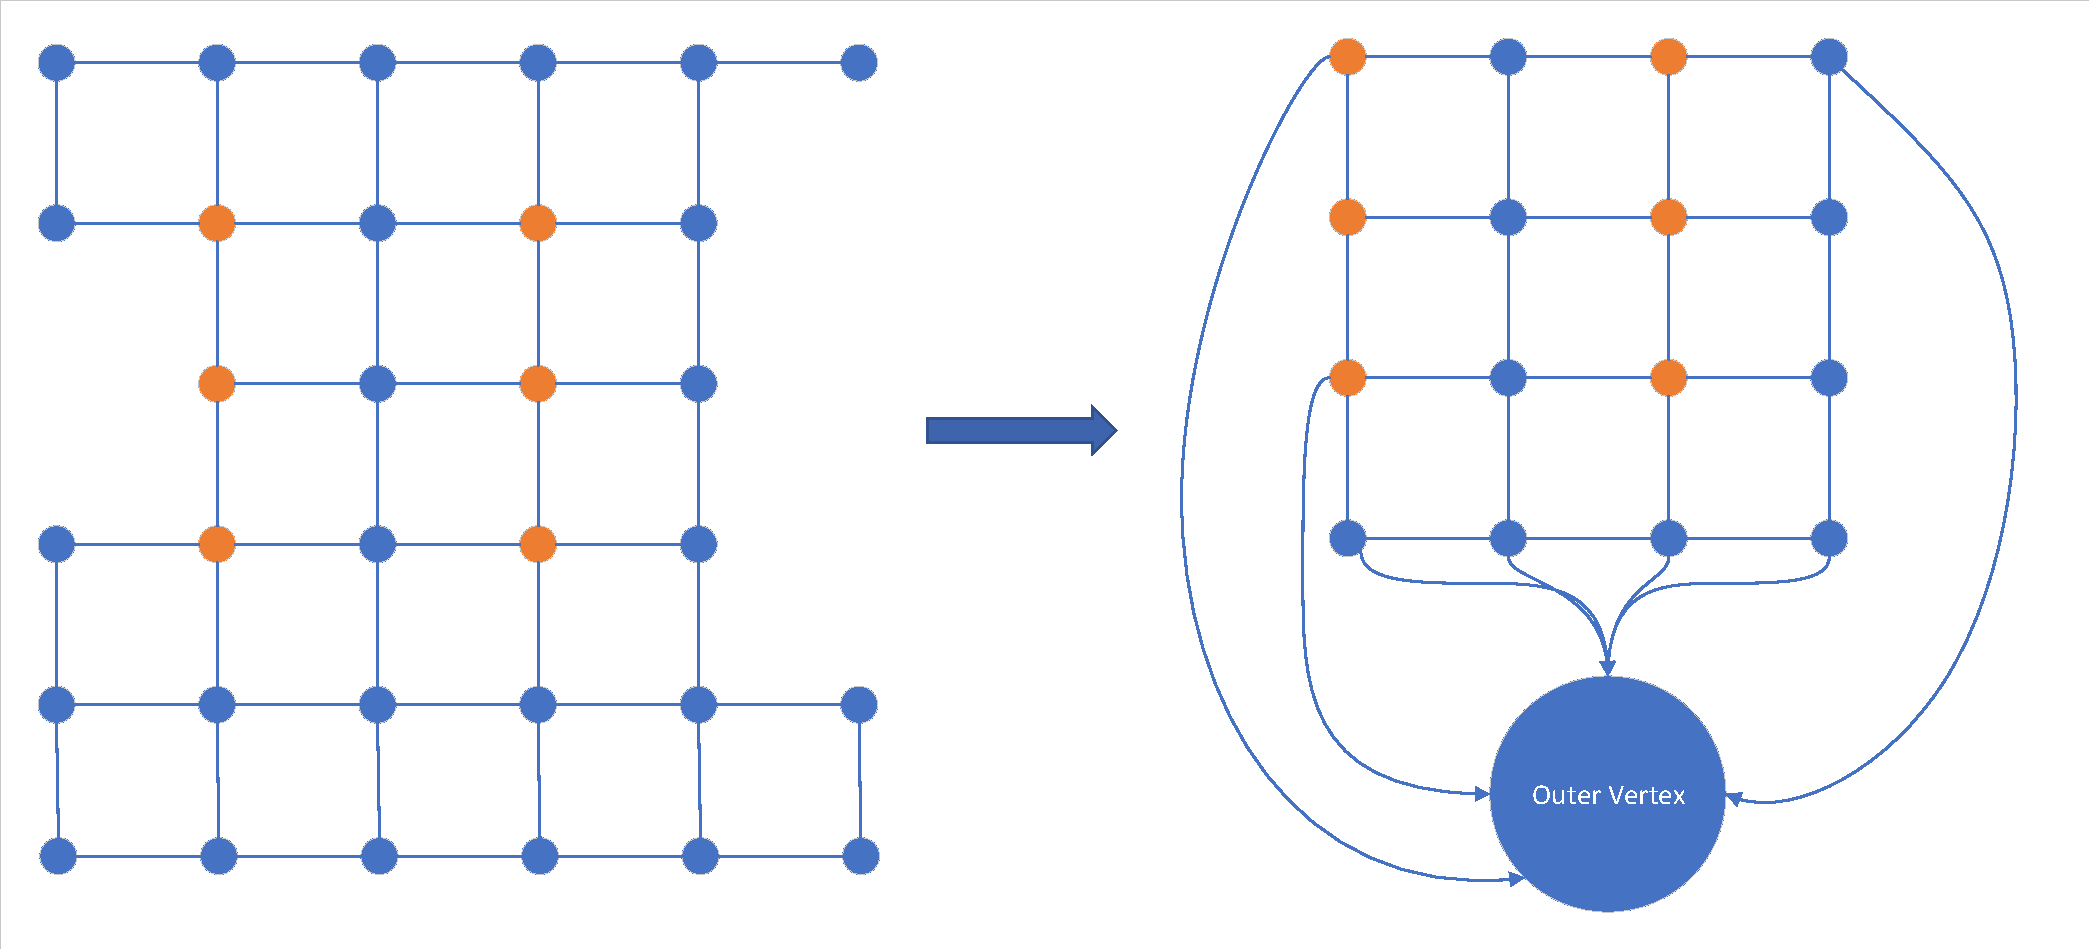
\includegraphics[width=0.5\textwidth]{Fig-P3T1STEP2.pdf}
	\caption{Step2: Abstract the boundary into one node.}
	\label{Fig-STEP2}
	\end{figure}
	
	\textbf{\textit{Step 3:}} Generalization, as is shown in Fig/~\ref{Fig-STEP3}.
	Each vertex is regarded as a vertex with capacity of one, and it is transformed into a generalized node by the method of the previous question.
	\\
	Furthermore, each undirected edge is transformed into two directed edges with opposite directions between the same pair of vertices. 
	\\
	Except for the $Outer\ Vertex$, there are $2(n-1)^2$ vertices left, since each remaining vertex is \emph{split} into two vertices. 
	\begin{figure}[!htbp]
	\centering
	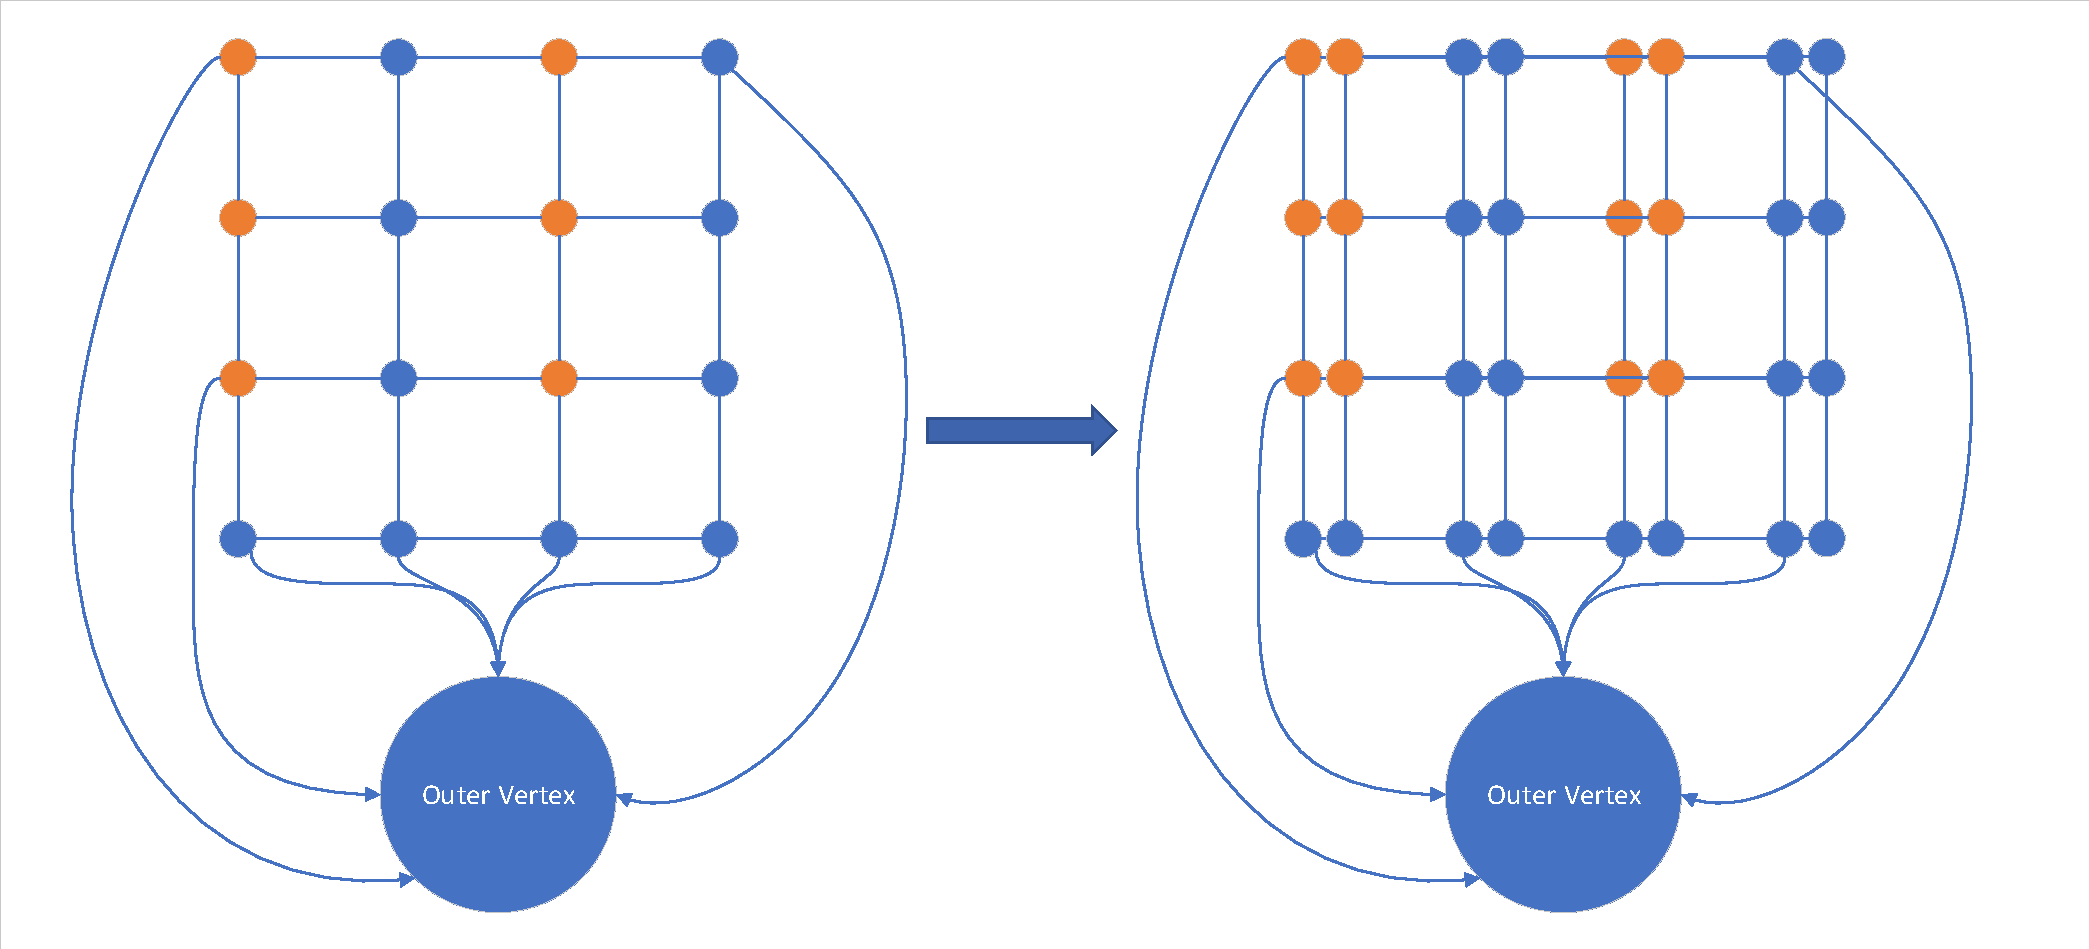
\includegraphics[width=0.5\textwidth]{Fig-P3T1STEP3.pdf}
	\caption{Step3: Generalization.}
	\label{Fig-STEP3}
	\end{figure}
	
	\textbf{\textit{Step 4:}} Solve the problem by modified Ford-Fulkerson algorithm.
	\\
	Let $V$ to denote the set of remaining vertices, $E$ to denote the set of directed edges, and $S$ to denote the set of remaining starting vertices.
	\\
	\begin{algorithm}[H]
	\caption{Solving escape problem}\label{Alg-SEP}
	\KwIn{$G=(V,E)$,$S$}
	\BlankLine
	
	\ForEach{$e\in E$}{
	    $f(e)\leftarrow 0$\;
	}
	$G_f\leftarrow$ residual graph\;
	$t\leftarrow Outer\ Vertex$\;
    \ForEach{$s\in S$}{
        \While{$An\ augmenting\ path\ P_{s,t}\ exists$}{
            $f\leftarrow AUGMENT(f,1,P)$\;
            update $G_f$\;
        }
    }
    capacity$\leftarrow$ flow\;
    \ForEach{$s\in S$}{
        \If{$the\ path\ from\ s\ to\ t\ doesn't\ exist$}{
        \Return{$False$\;}}
    }
    \Return{$True$\;}
	\end{algorithm}
	\textbf{\textit{Time complexity analysis:}}
	Considering the time complexity of searching a path(or augmenting path) is $O(|V|+|E|)$ and that of $Ford-Fulkerson$ algorithm is $O(|E|\times|V|)$, the time complexity of the $for$ loop in line 5 is $O(|S|\times|V|\times|E|)$. Furthermore, the time complexity of the $for$ loop in line 10 is $O(|S|\times (|V|+|E|))$. 
	
	As a result of this, the time complexity of the algorithm is $$O(|S|\times|V|\times|E|)$$
	Since $|S|=m$, $|V|=2(n-1)^2+1$, and $|E|\sim n^2$, the total time complexity is $$O(|S|\times|V|\times|E|)=O(mn^4)$$
    \end{enumerate}
    \end{solution}
    
    
    
\end{enumerate}

\textbf{Remark:} Please include your .pdf, .tex files for uploading with standard file names.
\newpage


%========================================================================
\end{document}